\section{Interface Graphique}
\label{interf_graph}
\subsection{Cahier des Charges spécifique} %-------------------------------
\begin{itemize}
    \item Sélection dynamique du fichier Lotus depuis l'explorateur de fichiers puisque ce fichier va changer très souvent (versionnement des fichiers Lotus, donc versionnement de la LAS de le voiture, se fait par enregistrement de différents fichiers) 
    \item Affichage des messages d'erreur et du résumé de mise à jour
    \item Bouton mise à jour de l'assemblage
    \item Sélection dynamique du fichier Catia depuis l'explorateur du fichier : mémoriser le parcours d'enregistrement des fichiers \texttt{WireframeDefinition.CATProduct} car il ne vont pas changer très souvent.
    \item donner la possibilité à l'utilisateur de sélectionner d'autres produits à mettre à jour après la mise à jour des points
    \item Conserver les derniers produits updatés lors de l'itération précédente, afin de faire gagner du temps à l'utilisateur lors des nombreuses itérations.
\end{itemize}


\subsection{Définition de l'interface} %----------------------------------
\begin{minipage}{\textwidth}
    \centering \vspace{1em}
    \includegraphics[height=10cm]{img/interfaceGraphique.pdf}
    \includegraphics[height=10cm]{img/interface.png}
    \captionof{figure}{Représentation schématique (gauche) et réalisation de l'interface (droite) de l'interface de la Macro}
    \label{fig:interfaceGraphique}
\end{minipage}

\\

\par La fig. \ref{fig:interfaceGraphique} présente la structure souhaitée pour l'interface de la Macro: trois sections se définissent.
\par Premièrement, on retrouve le champ pour la sélection du fichier Lotus \texttt{.dat} avec l'enregistrement de l'analyse cinématique.
\par Deuxièmement, on trouve le champ pour la sélection du Produit Catia pour la définition du filaire à partir des points. La macro va automatiquement repérer à l'intérieur de ce Produit la pièce \texttt{LotusPoints.CATPart} afin de mettre à jour les points. 
\par Troisièmement, on retrouve une section pour la sélection multiple des produits à mettre à jour suite au changement des points LAS : le choix est fait par l'utilisateur en fonction du travail demandé.

\par On remarque que l'utilisateur peut ne pas avoir besoin de changer tous les fichiers chaque fois puisque seulement le fichier \texttt{Lotus.dat} est sensé varier. On souhaiterait donc que cette application garde en mémoire les adresses des fichiers utilisés lors de la dernière utilisation tout en laissant à l'utilisateur la possibilité de les modifier en cas de besoin. Pour ce faire, un nouveau fichier \texttt{params.txt} est créé et mis à jour dans le même répertoire de stockage de la bibliothèque de la macro.

\par On remarque également que le bouton "Cancel" prévu dans la maquette de l'interface se matérialise dans le bouton de fermeture de la fenêtre de la macro.


\subsection{Enregistrement des dernières positions des fichiers} % ---------------------------------

\par Afin de simplifier l'utilisation de la macro, on décide de stocker la dernière valeur de la position du dernier fichier \texttt{WireframeDefinition.CATProduct} dans la première ligne du fichier \texttt{params.txt} et de laisser à l'utilisateur la possibilité de changer cette position à travers l'interface graphique. On implémentera la même solution pour l'ensemble des produits que l'utilisateur ajoutera dans le champ \textit{Other products to update} de l'interface graphique et également pour le dernier fichier Lotus utilisé, afin de pouvoir les charger la fois suivante à l'ouverture de la macro.

\par Afin de charger ces paramètres lors du lancement de l'application, on utilise la subroutine \texttt{UserForm\_Activate} et on implémente une simple lecture du fichier texte params.txt avec un objet de type \textit{TextStream}. Pour l'enregistrement des positions des fichiers avant la fermeture de l'application, on utilise la subroutine \textit{UserForm\_QueryClose} et on remplace tout simplement les nouvelles positions dans le fichier texte. La structure du fichier \texttt{params.txt} se définit donc de façon simple:
\begin{enumerate}
    \item path du dernier fichier \texttt{WireframeDefinition.CATProduct} dans la première ligne
    \item path du dernier fichier Lotus \texttt{.dat} dans la deuxième ligne
    \item path des derniers produits supplémentaires à mettre à jour à partir de la troisième ligne
\end{enumerate}

\par Ainsi, afin de n'écrire qu'une fois dans le fichier params.txt, étant donné que la manipulation d'un fichier txt en VBA est plutôt lourde, nous passons par l'intermédiaire d'un tableau, appelé \textit{update\_products} dans notre code,  tableau dans lequel nous ajoutons ou enlevons le path des produits ainsi ajoutés ou enlevés. Ensuite, nous copions termes à termes les paths dans params.txt à la fermeture de l'UserForm.

\subsection{Messages d'erreurs} % ---------------------------------------------------

\par Différentes erreurs sont pris en compte lors par cette Macro :

\begin{itemize}
    \item Si l'utilisateur oublie de renseigner la path d'un fichier Lotus et clique sur Update, la macro l'oblige à en choisir un
    \item Même méthode s'il oublie de choisir le path de \texttt{WireframeDefinition.CATProduct}.
\end{itemize}
